%!TeX program = pdflatex
\documentclass[12pt,a4paper]{report}
\usepackage[utf8]{inputenc}
\usepackage[T1]{fontenc}
\usepackage{helvet}
\usepackage{graphicx}
\usepackage{xcolor}
\usepackage{tikz}
\usetikzlibrary{positioning,shapes.geometric,arrows}

\geometry{left=2.5cm,right=2.5cm,top=2.5cm,bottom=2.5cm}

\begin{document}

\begin{center}
\Large\textbf{wFabricSecurity Architecture}\\[1cm]
\end{center}

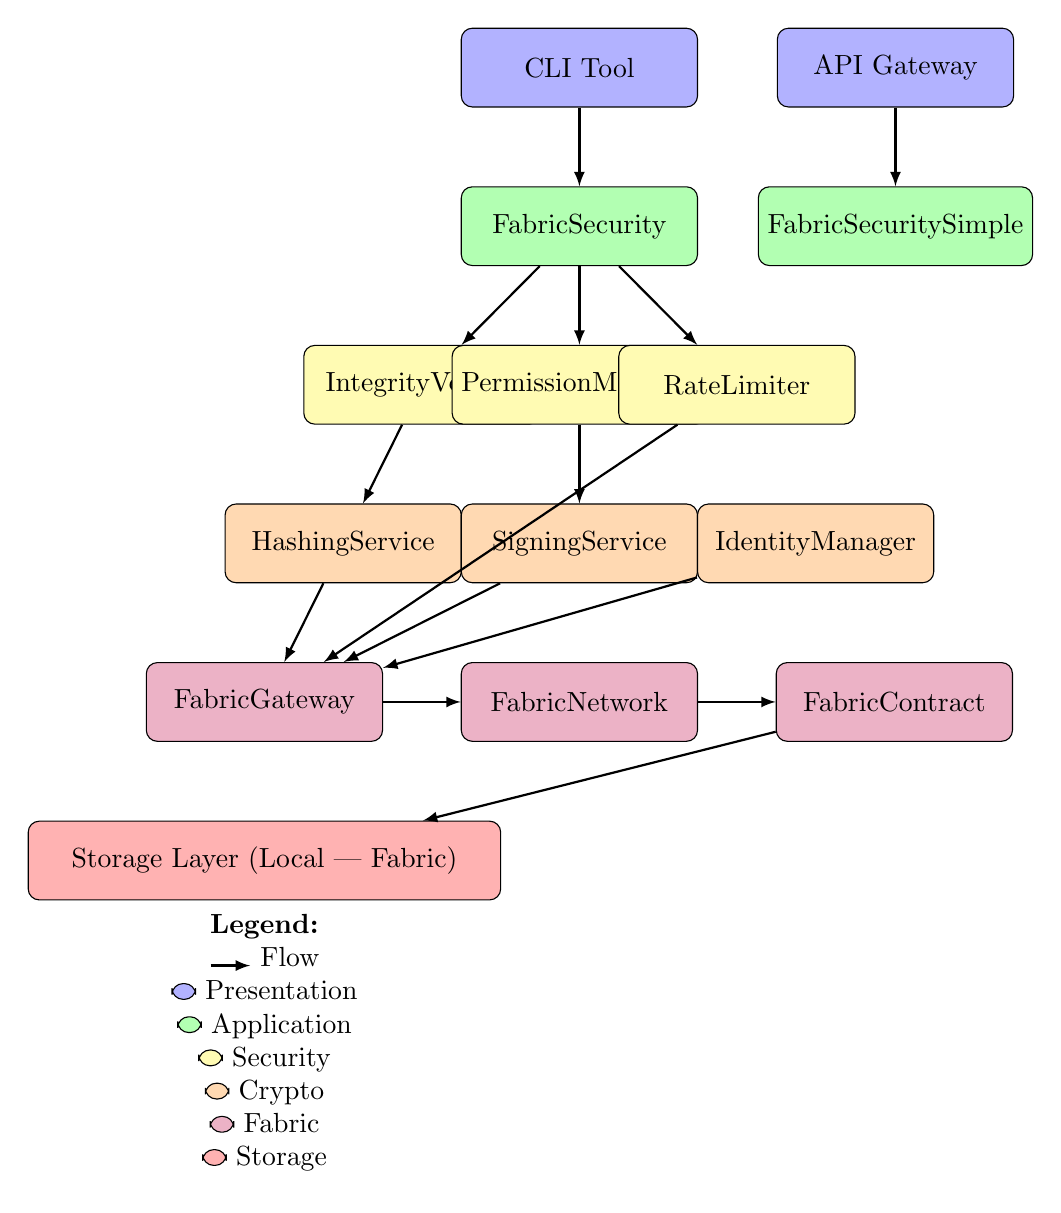
\begin{tikzpicture}[
    >=latex,
    node distance=1cm,
    block/.style={rectangle, draw, fill=blue!20, minimum width=3cm, minimum height=1cm, rounded corners},
    arrow/.style={->, thick},
    label/.style={text width=3cm, align=center}
]

% Presentation Layer
\node[block, fill=blue!30] (cli) {CLI Tool};
\node[block, fill=blue!30, right=of cli] (api) {API Gateway};

% Application Layer
\node[block, fill=green!30, below=of cli] (security) {FabricSecurity};
\node[block, fill=green!30, below=of api] (simple) {FabricSecuritySimple};

% Security Layer
\node[block, fill=yellow!30, below=of security, xshift=-2cm] (integrity) {IntegrityVerifier};
\node[block, fill=yellow!30, below=of security, xshift=0cm] (permissions) {PermissionManager};
\node[block, fill=yellow!30, below=of security, xshift=2cm] (rate) {RateLimiter};

% Crypto Layer
\node[block, fill=orange!30, below=of integrity, xshift=-1cm] (hashing) {HashingService};
\node[block, fill=orange!30, below=of permissions, xshift=0cm] (signing) {SigningService};
\node[block, fill=orange!30, below=of rate, xshift=1cm] (identity) {IdentityManager};

% Fabric Layer
\node[block, fill=purple!30, below=of hashing, xshift=-1cm] (gateway) {FabricGateway};
\node[block, fill=purple!30, below=of signing, xshift=0cm] (network) {FabricNetwork};
\node[block, fill=purple!30, below=of identity, xshift=1cm] (contract) {FabricContract};

% Storage Layer
\node[block, fill=red!30, below=of gateway, minimum width=6cm] (storage) {Storage Layer (Local | Fabric)};

% Arrows
\draw[arrow] (cli) -- (security);
\draw[arrow] (api) -- (simple);
\draw[arrow] (security) -- (integrity);
\draw[arrow] (security) -- (permissions);
\draw[arrow] (security) -- (rate);
\draw[arrow] (integrity) -- (hashing);
\draw[arrow] (permissions) -- (signing);
\draw[arrow] (rate) -- (gateway);
\draw[arrow] (hashing) -- (gateway);
\draw[arrow] (signing) -- (gateway);
\draw[arrow] (identity) -- (gateway);
\draw[arrow] (gateway) -- (network);
\draw[arrow] (network) -- (contract);
\draw[arrow] (contract) -- (storage);

% Legend
\node[below=of storage, yshift=1cm, anchor=north] {
    \begin{tabular}{c}
        \textbf{Legend:} \\
        \tikz\draw[->,thick] (0,0) -- (0.5,0); Flow \\
        \tikz\draw[block, fill=blue!30] (0,0) rectangle (0.3,0.2); Presentation \\
        \tikz\draw[block, fill=green!30] (0,0) rectangle (0.3,0.2); Application \\
        \tikz\draw[block, fill=yellow!30] (0,0) rectangle (0.3,0.2); Security \\
        \tikz\draw[block, fill=orange!30] (0,0) rectangle (0.3,0.2); Crypto \\
        \tikz\draw[block, fill=purple!30] (0,0) rectangle (0.3,0.2); Fabric \\
        \tikz\draw[block, fill=red!30] (0,0) rectangle (0.3,0.2); Storage \\
    \end{tabular}
};

\end{tikzpicture}

\vfill

\begin{center}
\textbf{wFabricSecurity - Zero Trust Security System}\\[0.5cm]
\today
\end{center}

\end{document}
